Based on the experiences made for \cite{preibisch2014efficient, schmid2015real}, this section will discuss results obtained with \gearshifft{} on various hardware in order to showcase the capabilities of \gearshifft{}. We will assume the motivation of a developer seeking to optimize the use of FFTs in the context of the aforementioned publications, i.e. 3D real-to-complex transforms with contiguous single-precision input data. If not stated otherwise, this is the transform type assumed for all illustrations hereafter. 

Expeditions into other use cases will be made where appropriate. The curious reader may rest assured that a more comprehensive study is easily possible with \gearshifft{}, however the mere multiplicity of all possible combinations and use cases of FFT render it neither feasible nor practical to discuss 1D or 2D in a comprehensive fashion as well.

For this study, we will concentrate on three modern and current FFT implementations available free of charge: FFTW ($3.3.5$, on x86 CPUs), cuFFT ($8.0.44$, on nVidia GPUs) and clFFT ($2.12.2$, on x86 CPUs or nVidia GPUs). We consider this the natural starting point of developers beyond possible domain specific implementations. It should be noted, that this will infer not only a study in terms of hardware performance, but also how well the APIs designed by the authors of FFTW, clFFT and cuFFT are documented, understood and used in practice. We consider both hardware and cognitive/developer performance a virtue of equal importance.

\subsection{Experimental Environment}
\label{ssec:env}

The results presented in the following sections were collected on three systems:

\begin{itemize}
\item \emph{Taurus HPC cluster}\cite{taurus} running RHEL 7.2
  \begin{itemize}
  \item \emph{K80 node}: 2x Intel(R) Xeon(R) CPU E5-2680 v3 (12 cores) @ 2.50GHz, 64 GB RAM, 4x NVIDIA Tesla K80 (12 GB GDDR5 RAM) GPUs 
  \item \emph{K20X node}: 2x Intel(R) Xeon(R) CPU E5-2450 (8 cores) @ 2.10GHz, 48 GB RAM, 2x NVIDIA Tesla K20x (6 GB GDDR RAM) GPUs 
  \end{itemize}
\item \emph{Hypnos HPC cluster}\cite{hypnos} running Ubuntu 14.04.3:\newline
  2x Intel(R) Xeon(R) CPU E5-2603 v3 @ 1.60GHz, 64 GB RAM (2.67 GB per core), 1x NVIDIA Tesla P100 (16 GB HBM2 RAM) GPUs via PCIe 
\item  \emph{Dell workstation} running CentOS 7.2:\newline 
  2x Intel(R) Xeon(R) CPU E5-2640 v3 @ 2.60GHz, 64 GB RAM, 1x NVIDIA GeForce GTX 1080 (8 GB GDDR5X RAM)
\end{itemize}

As presented above, all used systems operated on a variant of 64-bit Linux and were accessed via an ssh session without running a graphical user interface of any kind. All measurements used the GNU compiler collection (GCC, \cite{stallman2001using}) version 5.3.0 as the underlying compiler if not stated otherwise. All used GPU implementations on nVidia hardware interfaced with the proprietary driver provided by the vendor $367.48$ (K20Xm, K80, P100) and $367.57$ (GTX1080). 

In order to generate one data set, a set arrays of arbitrary shapes is provided to a specific FFT API. The configuration files thereof can be accessed via \cite{gearshifft_github}. The shape configurations are separated in groups: \texttt{powerof2} (all dimensions are powers of $2$), \texttt{radix357} (all dimensions are either powers of $3$, $5$ or $7$) and \texttt{oddshape} (all dimensions are powers of $19$ in order to emulated very uncommon signal sizes). These configurations were generated in order to probe the FFT implementations for a wide spectrum of possible applications.  

The FFT calls to benchmark are executed five times each. From this, the arithmetic mean and sample standard deviations are used for figures presented below. As the number of repetitions is a configurable parameter of \gearshifft{}, we leave it to the user to produce a more comprehensive data set than used for this publication. We consider five repetitions enough at this point to show and discuss several aspects of performance and usability of \gearshifft{} and the FFT libraries under study.  

%TODO: why maximum size of transforms?

\subsection{Time To Solution}
\label{ssec:tts}

We begin the discussion with the classical use case for developers that might be accustomed to small size transforms. As such, an out-of-place transform with \texttt{powerof2} signal shapes will be assumed. The memory volume required for this operation amounts to the real input array plus an equally shaped complex output array.   

\begin{figure}[!tbp]
  \centering
  
\includegraphics[width=\textwidth]{figures/results_figure1_legend.pdf}
  \subfloat[Fig A.]{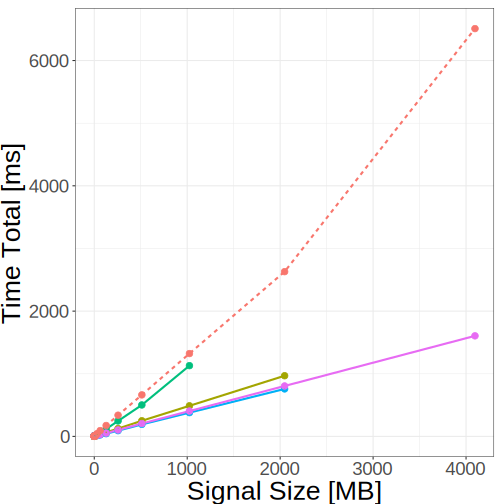
\includegraphics[width=0.45\textwidth]{figures/results_figure1a.pdf}\label{fig:f1a}}
  \hfill
  \subfloat[Fig B.]{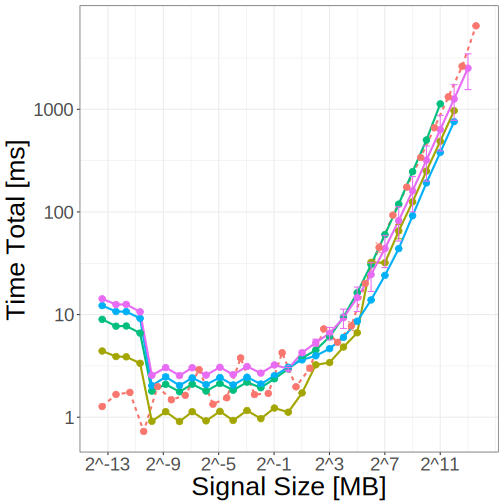
\includegraphics[width=0.45\textwidth]{figures/results_figure1b.pdf}\label{fig:f1b}}
  \caption{Time-to-solution for power-of-2 3D single-precision real-to-complex forward transforms using FFTW (\texttt{FFTW\_ESTIMATE}) and cuFFT. \cref{fig:f1b} shows the same data as \cref{fig:f1a} but in a log10-log2 scale.}
  \label{fig:tts}
\end{figure}

\cref{fig:tts} reports a comparison of runtime results of power-of-2 single-precision real-to-complex forward transforms from FFTW and cuFFT. It is evident that given the largest device memory available of  \SI{16}{\gibi\byte}, the GPU data does not yield any points higher than \SI{8}{\gibi\byte}. Note that the total time reflects the time to set up a plan, allocate memory on device, perform the data transfer onto the device, execute the FFT, transfer the result back to the host and clean up the used plan and the allocated memory. \cref{fig:f1a} shows that the oldest GPU generation used in this comparison yields the slowest results for input signals in the order of \SIrange{1}{2}{\gibi\byte}. All other and more recent GPU models supersede FFTW using all available cores in this node. Any judgment on the superiority of cuFFT over FFTW can be considered premature at this point, as FFTW was used with the \texttt{FFTW\_ESTIMATE} planner flag.

\begin{figure}[!tbp]
  \centering
  
\includegraphics[width=\textwidth]{figures/results_figure2_legend.pdf}
  \subfloat[Fig A.]{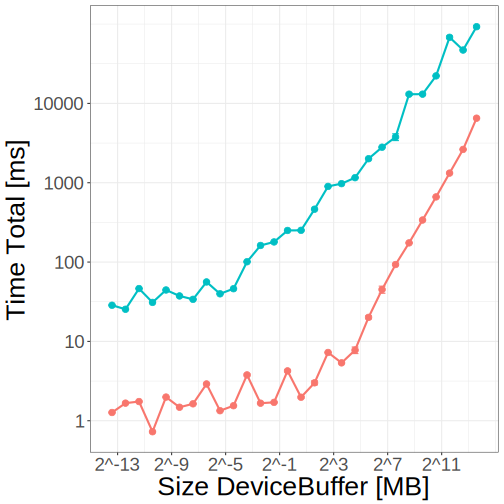
\includegraphics[width=0.45\textwidth]{figures/results_figure2a.pdf}\label{fig:f2a}}
  \hfill
  \subfloat[Fig B.]{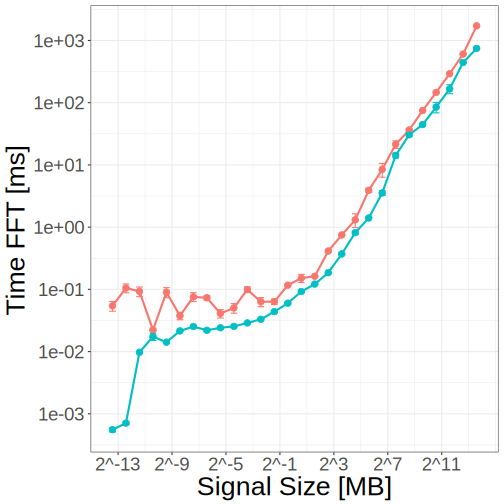
\includegraphics[width=0.45\textwidth]{figures/results_figure2b.pdf}\label{fig:f2b}}
  \caption{Time-to-solution for power-of-2 3D single-precision real-to-complex forward transforms using FFTW (\texttt{FFTW\_ESTIMATE}) and cuFFT. \cref{fig:f2a} report the complete time to solution, whereas \cref{fig:f2b} is limited to the time spent for the execution of the forward transform only. Both figures use a in a log10-log2 scale.}
  \label{fig:fftw_plan_flags}
\end{figure}

\cref{fig:fftw_plan_flags} compares the time-to-solution to the actual time spent for the FFT operation itself. This illustration makes the cost and the benefit of higher planning flags than \texttt{FFTW\_ESTIMATE} obvious. Where \texttt{FFTW\_MEASURE} imposes a runtime penalty of 1 to 2 orders of magnitude with respect to \texttt{FFTW\_ESTIMATE}, it offers superior performance. The careful observer has noticed that the planning times for \texttt{FFTW\_MEASURE} become prohibitively large for large input data sizes and reach minutes for data sets in the Gigabyte range. This is a well-known feature of FFTW as the authors note in \cite{FFTW05}:

\begin{center}
  ``In performance critical applications, many transforms of the same
  size are typically required, and therefore a large one-time cost is
  usually acceptable.''
\end{center}
 
\gearshifft{} allows to dissect this problem further and isolate the planning time only.

\begin{figure}[!tbp]
  \centering
  \subfloat[Fig A.]{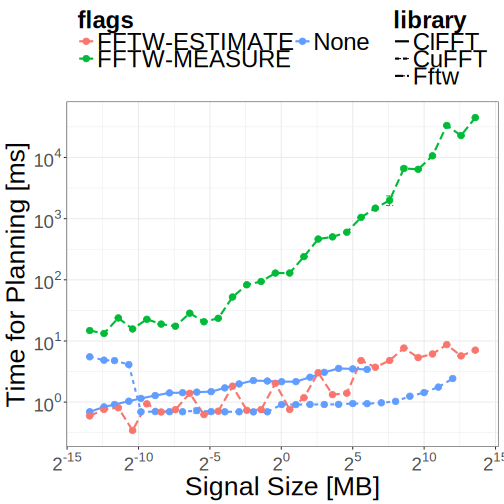
\includegraphics[width=0.45\textwidth]{figures/results_figure3a.pdf}\label{fig:f3a}}
  \hfill
  \subfloat[Fig B.]{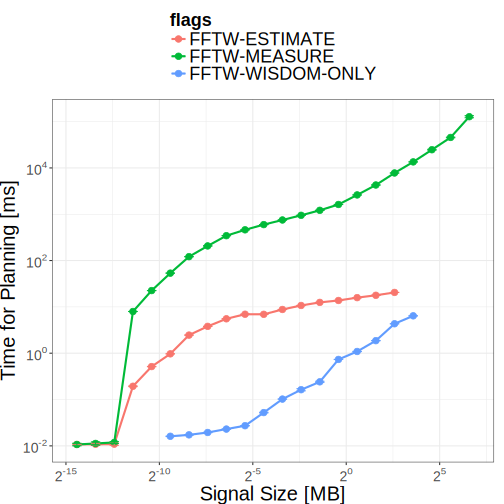
\includegraphics[width=0.45\textwidth]{figures/results_figure3b.pdf}\label{fig:f3b}}
  \caption{Time-to-plan for power-of-2 single-precision real-to-complex forward transforms using FFTW, cuFFT and clFFT. \cref{fig:f3a} reports the complete time to plan for 3D transforms, whereas \cref{fig:f3b} is limited to 1D transforms. Both figures use a log10-log2 scale.}
  \label{fig:plan_time_only}
\end{figure}

\cref{fig:plan_time_only} illustrates the problem to it's full extent. \texttt{FFTW\_MEASURE} consumes up to 3-4 orders of magnitude more time to produce a plan than a standard (GPU based libraries) or \texttt{FFTW\_ESTIMATE} based planner call especially for large input shapes, see \cref{fig:f3a}. We observed that FFTW wisdom cannot be generated for 2D or 3D out-of-place transforms. Therefor, we compare the 3D planning with it's counterpart in 1D in \cref{fig:f3b}. At input sizes of \SI{128}{\mebi\byte} in 1D, the planning phase exceeds the duration of \SI{100}{\second}. In practice, this imposes a challenge on the client to the FFTW API. Not only is the time to solution affected by this behavior which is a crucial quantity if FFT-heavy applications are run in an HPC environment. Here the runtime of applications needs to be know to some extent in order to allow efficient and rapid job placement in a cluster. Further, the developer interfacing with FFTW has to create infrastructure (thread-safe static singleton objects or similar come to mind) in order to perform the planning of FFTW only once and reuse the resulting plan as much as possible.

\subsection{Comparing CPU versus GPU runtimes}
\label{ssec:cpu_vs_gpu}

The last section finished by discussing a design artifact, that the FFTW authors introduced in their API and which the other FFT libraries discussed here adopted. Another important question typically asked is if GPU accelerated FFT implementations are really faster than their CPU equivalents. Although this question cannot be answered comprehensively in our study, we would like to point out several aspects of it. First of all, modern GPU are connected via the PCIe bus to the host system in order to transfer data, receive instructions and to be supplied with power. This imposes a severe bottleneck to data transfer and is sometimes neglected during library design. 

\begin{figure}[!tbp]
  \centering
  
\includegraphics[width=\textwidth]{figures/results_figure4_legend.pdf}
  \subfloat[cuFFT 8.0.44]{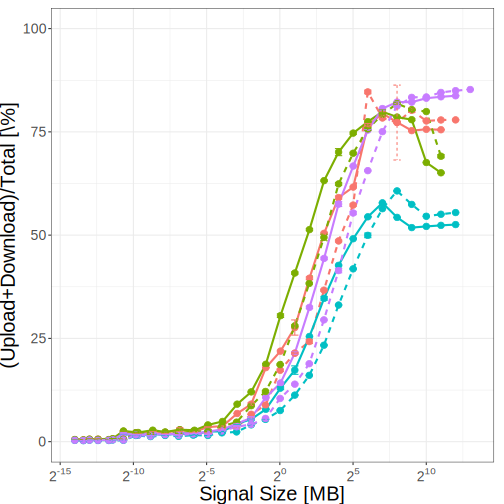
\includegraphics[width=0.45\textwidth]{figures/results_figure4a.pdf}\label{fig:f4a}}
  \hfill
  \subfloat[clFFT 2.12.2]{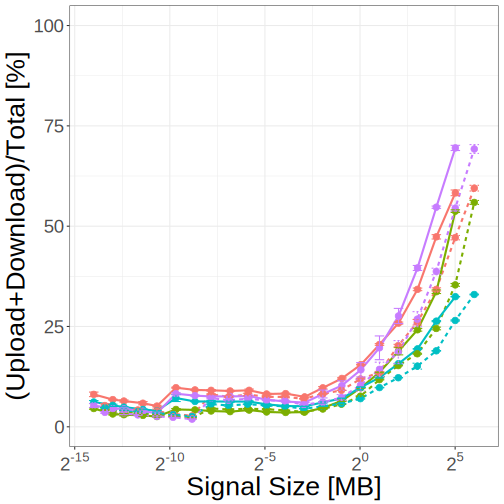
\includegraphics[width=0.45\textwidth]{figures/results_figure4b.pdf}\label{fig:f4b}}
  \caption{Time for upload plus time for download divided by the total time needed measured for power-of-2 single-precision real-to-complex forward transforms using cuFFT \cref{fig:f4a} and clFFT \cref{fig:f4b}. Both figures use a linear-versus-log2 scale.}
  \label{fig:device_transfer}
\end{figure}

\cref{fig:device_transfer} compares the time consumed by upload and download of input and output data for inplace and out-of-place FFT transforms using cuFFT \cref{fig:f4a} and clFFT \cref{fig:f4b}. It is not surprising to see that the ratio of transfer times amounts to up to \SIrange{75}{80}{\percent} for large input data sizes for cuFFT. This is caused by the use of paged memory for the input and output buffers. This forces the operating system and hence the GPU driver to check if the a given memory page needs to be stored to disk or not before it can be written or read. This introduces a severe overhead on the PCIe transfer. The reason for this choice was comparability during the design phase of \gearshifft{}. Using pinned or page-locked memory in CUDA is straight forward, doing the same in OpenCL is challenging and must be postponed to future releases. Another observation of \cref{fig:device_transfer} is that the measured runtimes become subject to stronger jitter  which is due to the host system mediating the transfer across the system hardware. As more software and hardware components are involved, these stochastic fluctuations accumulate. 

Besides the use of paged memory in \gearshifft{} which is not optimal in terms of performance but the natural choice for novice programmers, \cref{fig:device_transfer} illustrates that with increasing input signal size, the memory transfer can become a bottleneck. This still holds even if pinned or page-locked memory is used \cite{steinbach_gtc2015}.

\begin{figure}[!tbp]
  \centering
  
\includegraphics[width=\textwidth]{figures/results_figure5_legend.pdf}
  \subfloat[3D transforms]{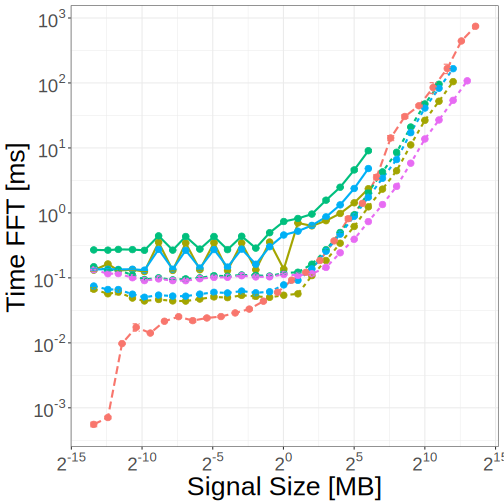
\includegraphics[width=0.45\textwidth]{figures/results_figure5a.pdf}\label{fig:f5a}}
  \hfill
  \subfloat[1D transforms]{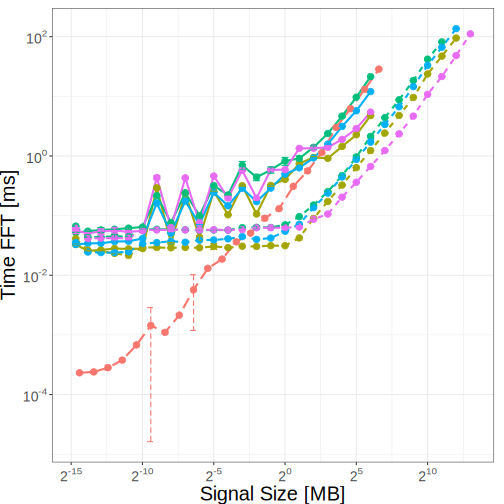
\includegraphics[width=0.45\textwidth]{figures/results_figure5b.pdf}\label{fig:f5b}}
  \caption{Time for computing power-of-2 single-precision real-to-complex forward transforms using the 3D API \cref{fig:f5a} and the 1D API clFFT \cref{fig:f5b}. Both figures use a log10-versus-log2 scale.}
  \label{fig:r2c_fwd}
\end{figure}

\cref{fig:r2c_fwd} shows the runtime spent for computing only the forward FFT for real single precision input data. This illustration is a direct measure for the quality of the implmentation and the hardware underneath. For the 3D case in \cref{fig:f5a}, we see that at the time of writing, FFTW on a double socket Haswell Intel Xeon E5 CPU provides very compelling performance if the input data is not larger than \SI{1}{\mebi\byte}. Above this limit, the GPU implementations offer a clear advantage by up to one order of magnitude. The current Pascal generation GPUs used with cuFFT provide the best performance, which does not come by surprise as both cards are equipped with GDDR5X or HBM2 memory which are clearly beneficial for an operation that yields low computational complexity such as the FFT. In the 1D case of \cref{fig:f5b}, the same observations must be made with even more certainty. The cross-over of FFTW and the GPU libraries occurs at an earlier point of \SI{64}{\kibi\byte}.  

\subsection{Non-power-of-2 transforms}
\label{ssec:nonpowerof2}

\subsection{Memory Modes}
\label{ssec:mem_mode}

\subsection{Data Types}
\label{ssec:data_types}

